\chapter{测试平台硬件架构}
\label{cha:Hardware}

\section{平台选型}

我们选用Nvidia Jetson NANO(如图~\ref{fig:Jetson-Nano})作为主要的开发平台,NVIDIA Jetson Nano开发人员工具包是一台功能强大的小型计算机,可并行运行多个神经网络,以用于图像分类,对象检测,分段和语音处理等应用,该平台的功耗仅为5瓦。

\begin{figure}[htbp] % use float package if you want it here
    \centering
    \includegraphics[height=6cm]{Jetson-Nano.jpg}
    \caption{Nvidia Jetson NANO}
    \label{fig:Jetson-Nano}
\end{figure}

初步的硬件平台,采用无线局域网通信,图~\ref{fig:wifi}为将AC8265和片状5GHz天线装到Jetson Nano Developer Kit上。

\begin{figure}[htbp]
    \begin{minipage}{0.48\textwidth}
      \centering
      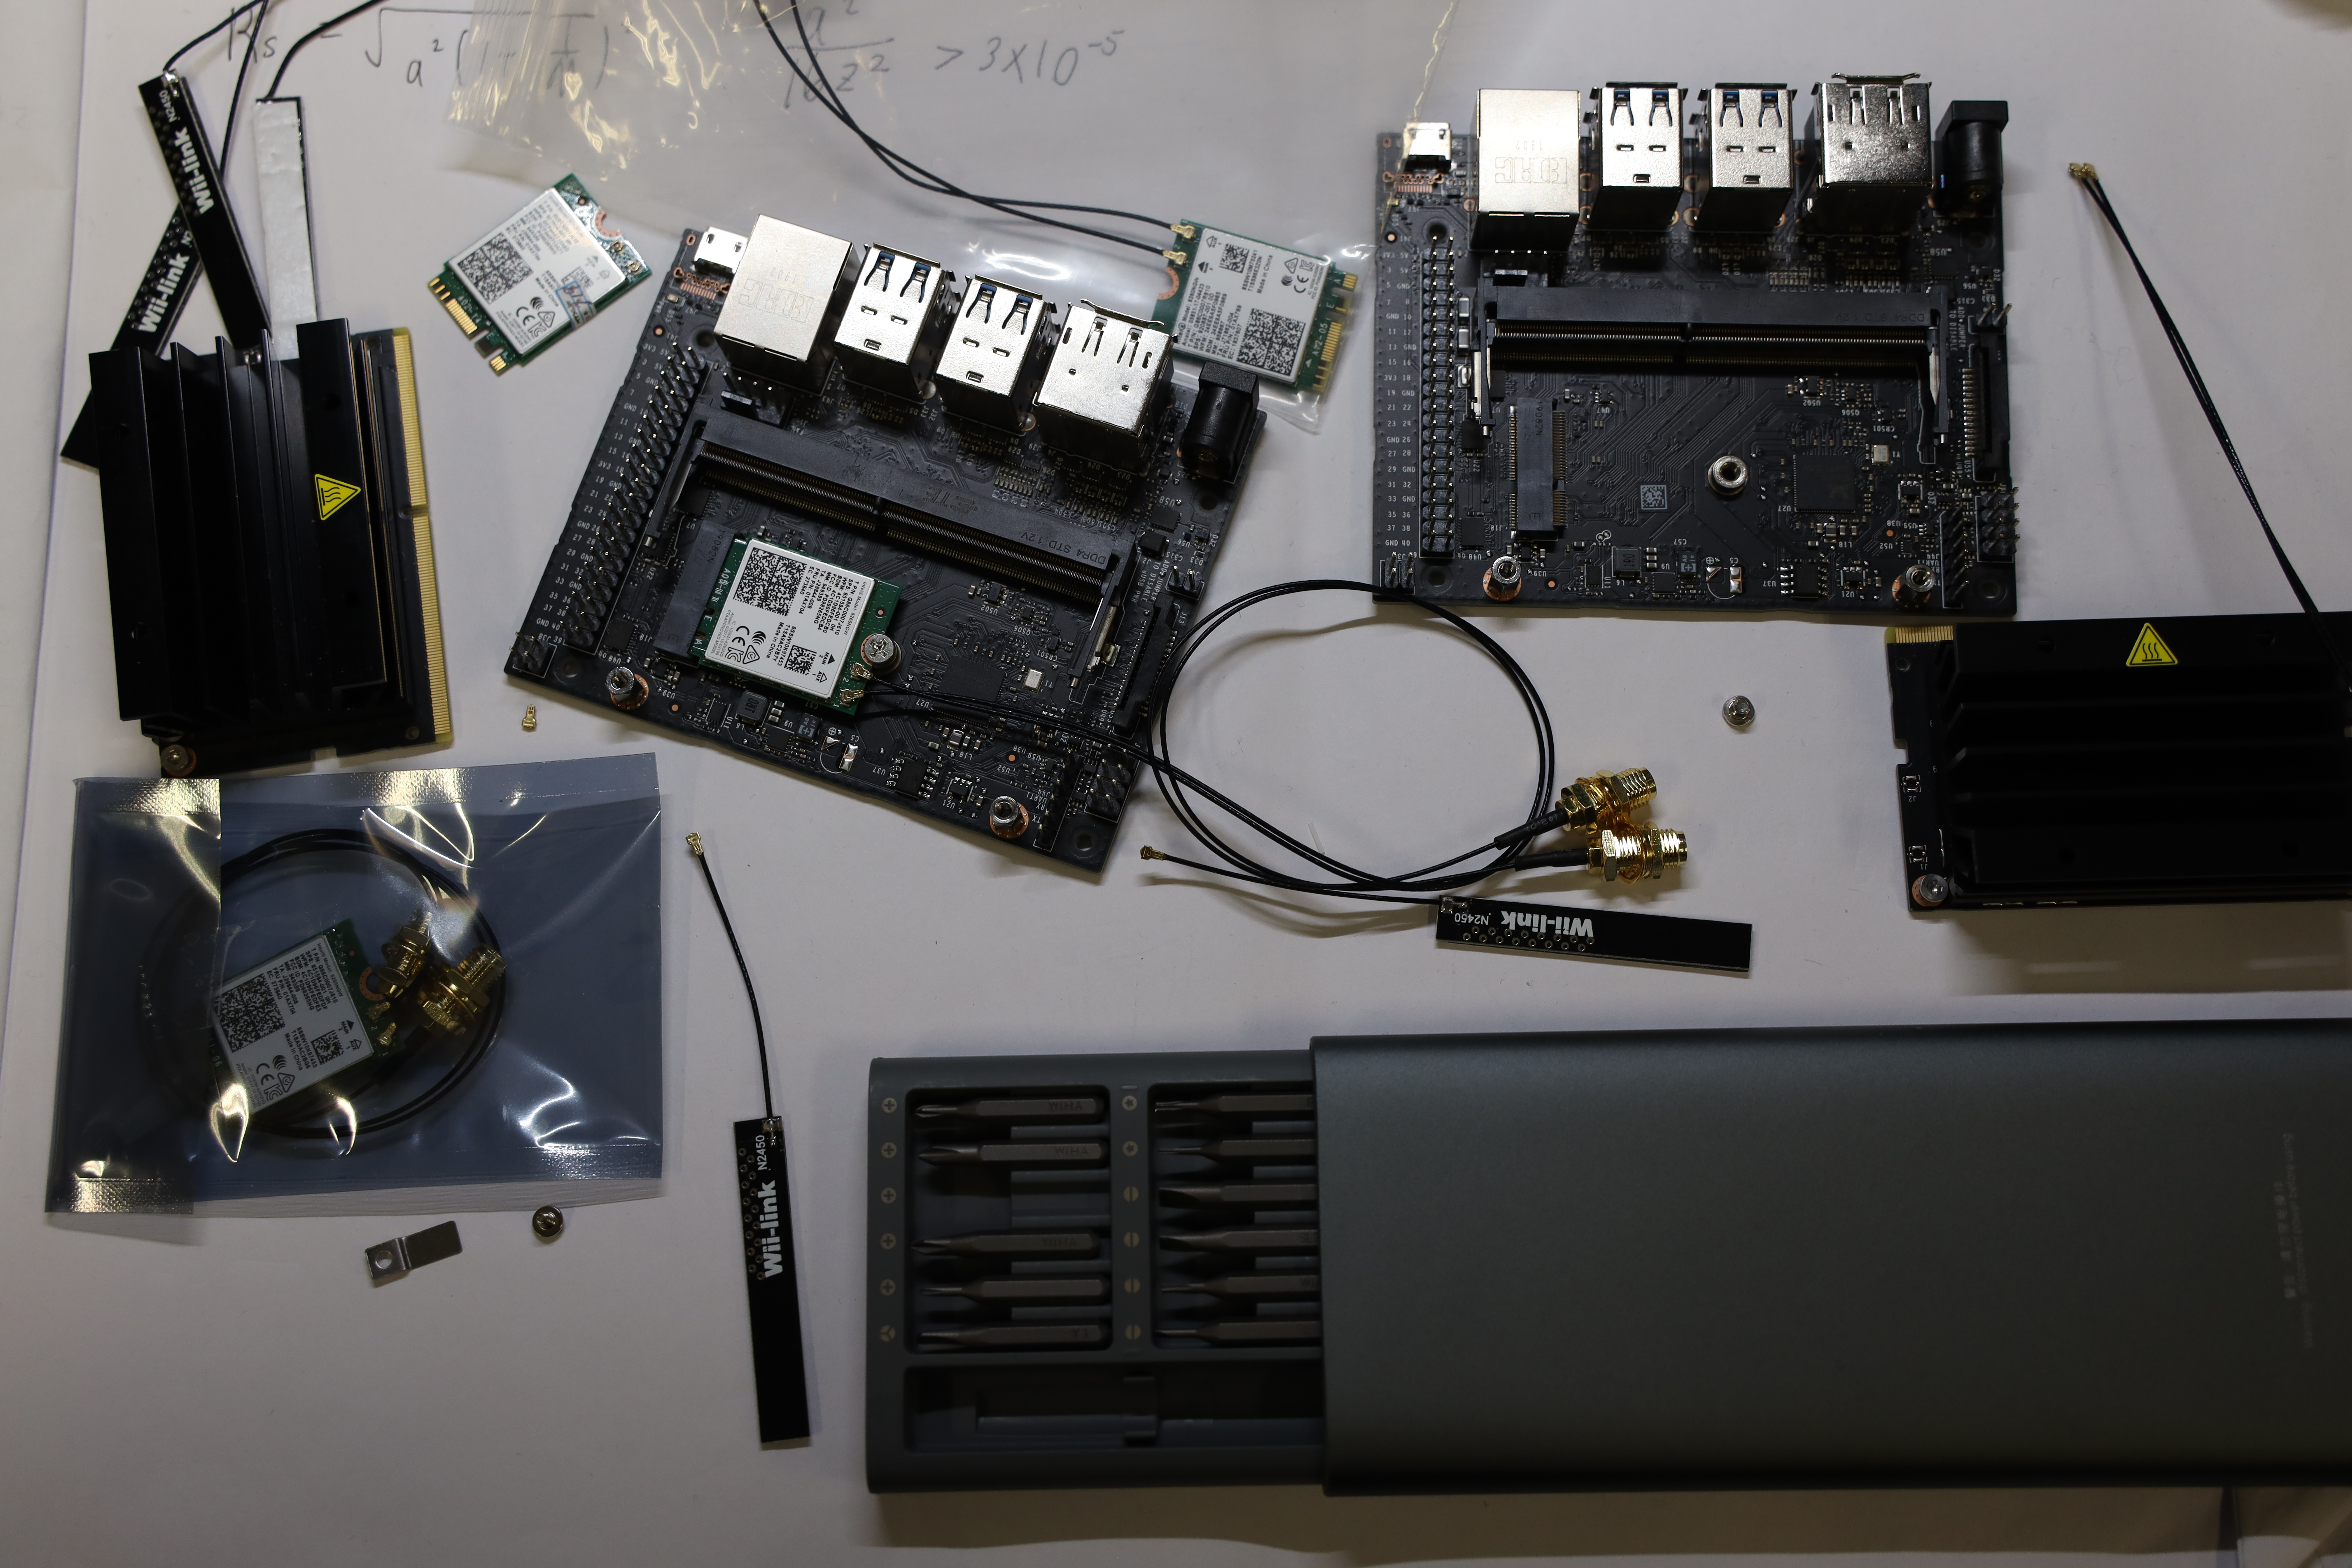
\includegraphics[height=5cm]{DA4A3052.JPG}
      \caption{为Nano添加无线网功能}
      \label{fig:wifi}
    \end{minipage}\hfill
    \begin{minipage}{0.48\textwidth}
      \centering
      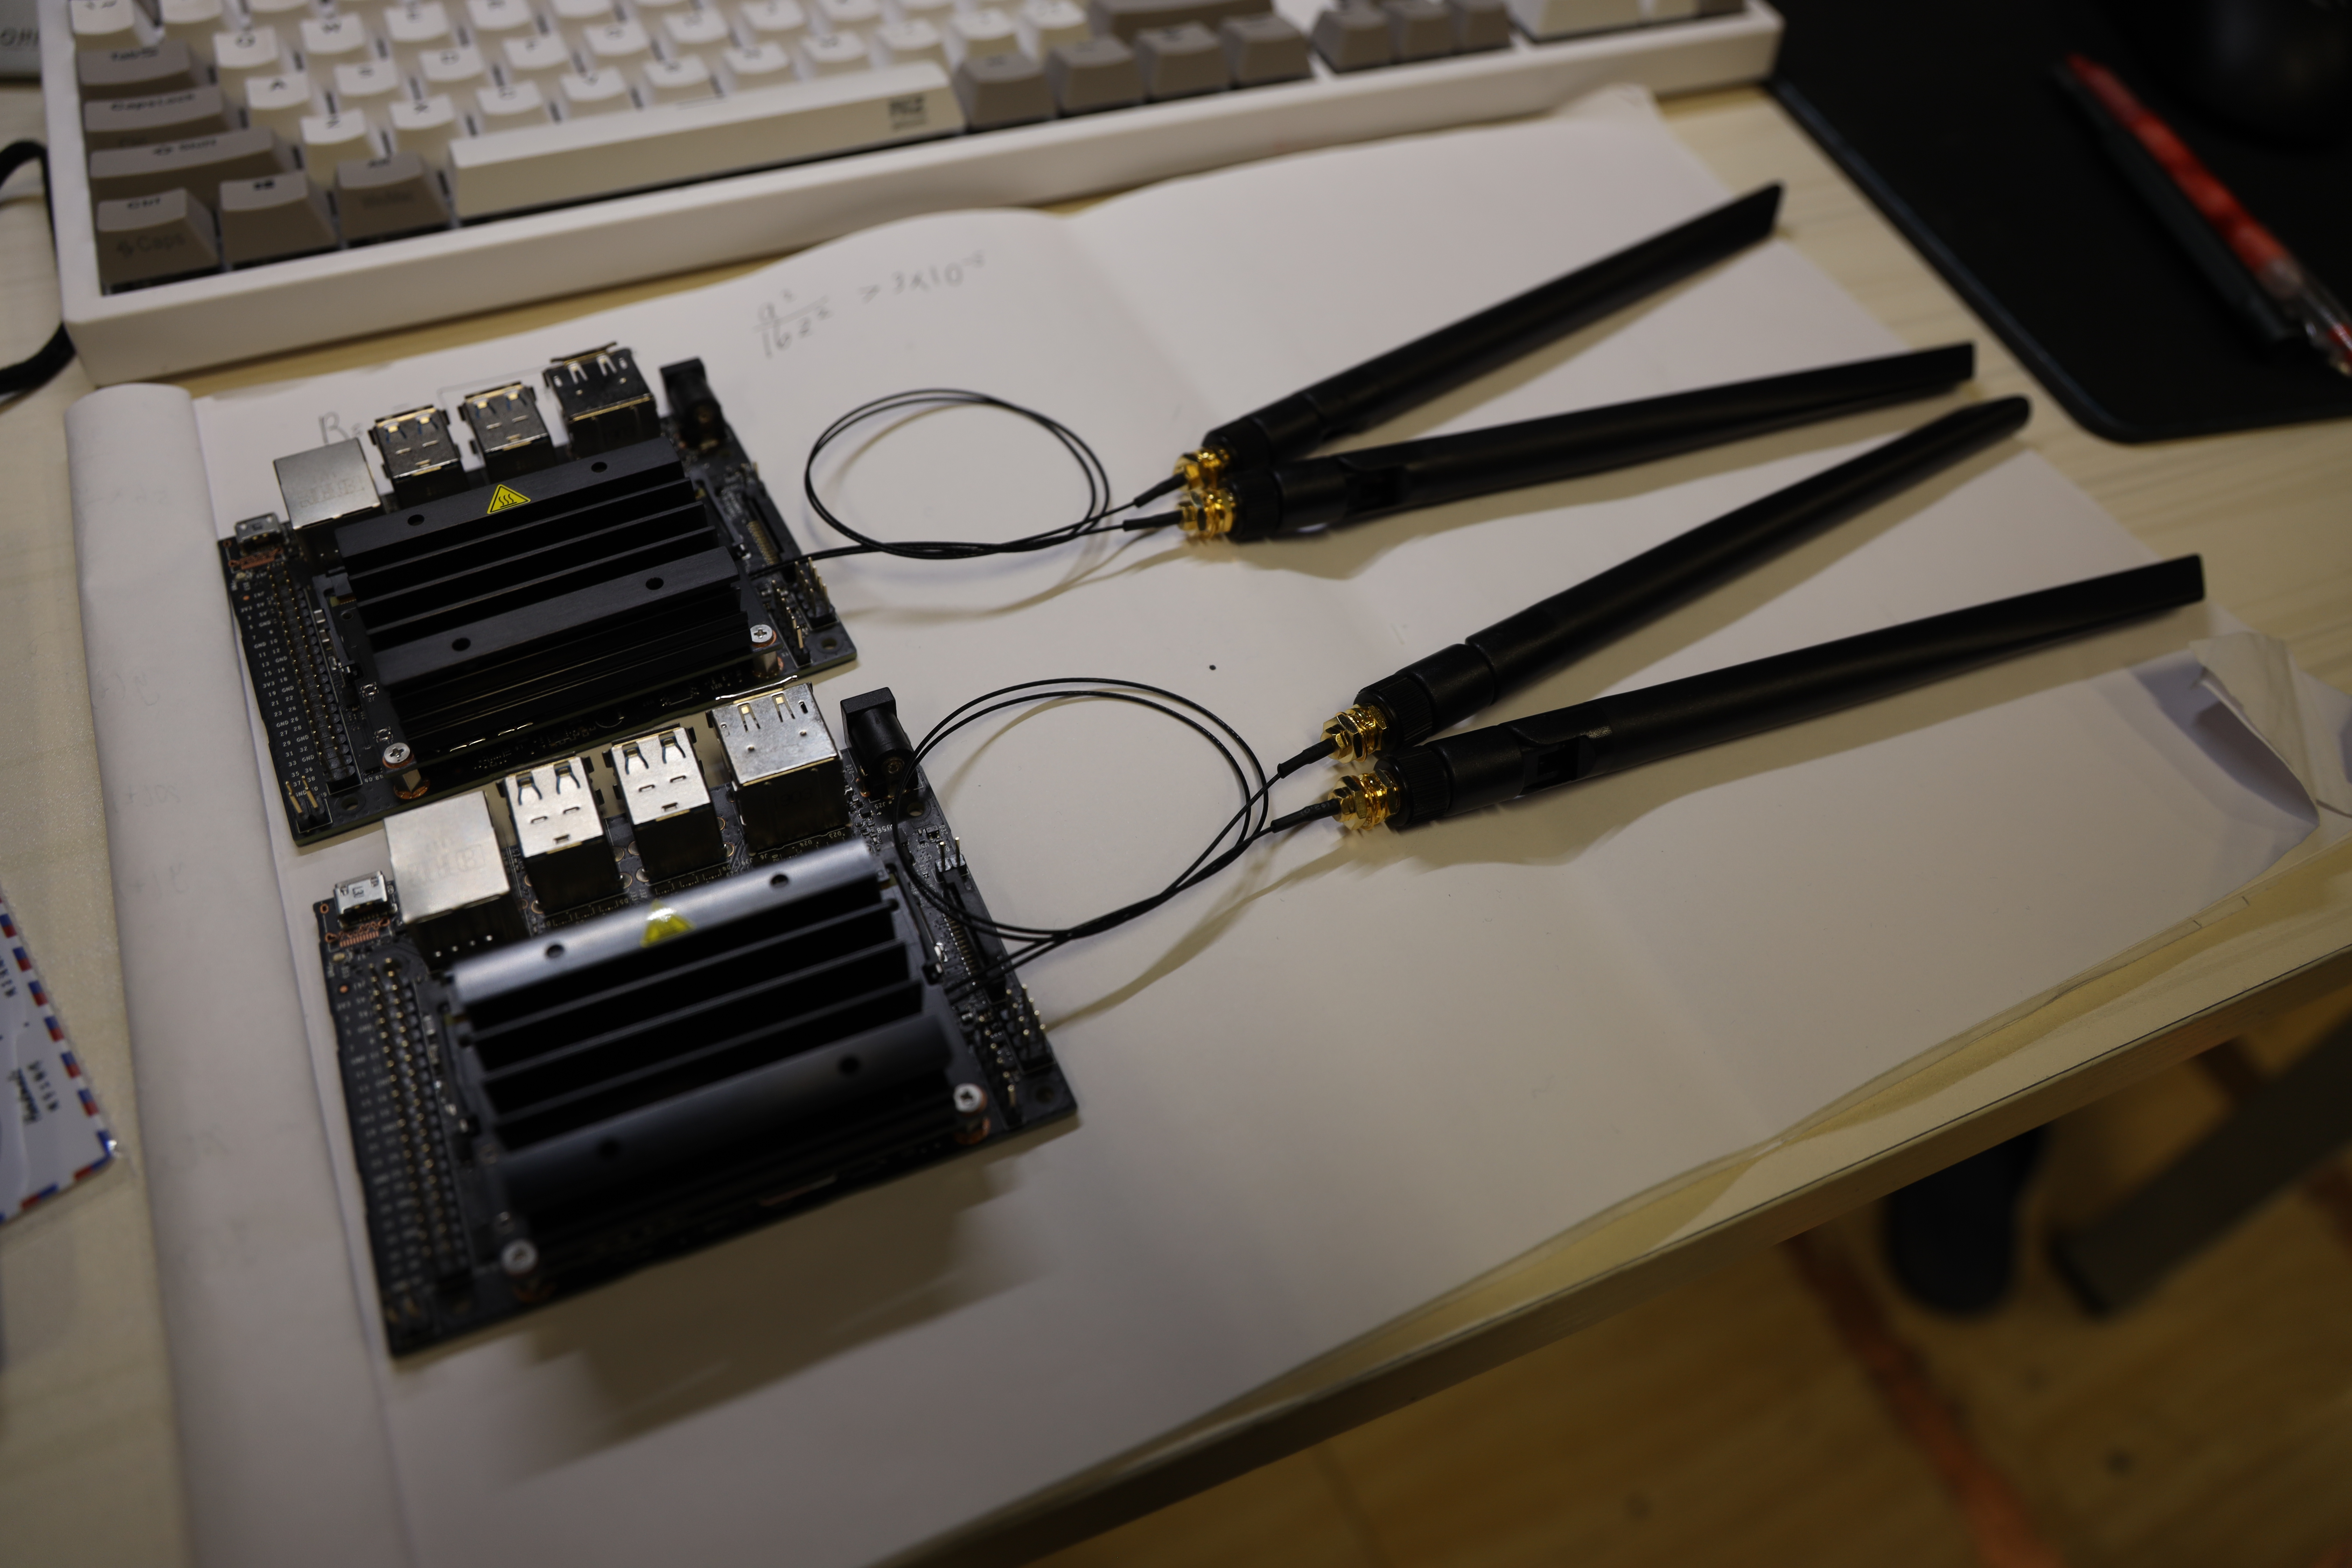
\includegraphics[height=5cm]{DA4A3066.JPG}
      \caption{两机组通信测试平台}
      \label{fig:two-setup}
    \end{minipage}
\end{figure}


\section{环境配置}